\section{Variance decomposition in the APE and IPM framework}
\label{app:var}
In the main text, we limited ourselves to a discussion of the absolute contributions of the different terms of the APE and IPM to the changes in mean trait value. Another focus of interest is to analyse which constituents underlie the biggest variance in this change. In the application of age-structured Price equation (APE) by \cite{Ozgul2009} on the sheep population on St. Kilda, both the absolute contributions to $\Delta \overline z$ over time and a variance partitioning of $\Delta \overline z$ into contributions were regarded. This partitioning aims at finding which processes cause \textit{changes} in $\Delta \overline z$ and is thus not directly comparable with contributions to changes in $\overline z$ (or: $\Delta \overline z$ itself). We have performed a variance partitioning for both the APE and integral projection model (IPM) approach by means of an ANOVA type III (Fig. \ref{app:var:fig1}).

\begin{figure}[H]
\centering
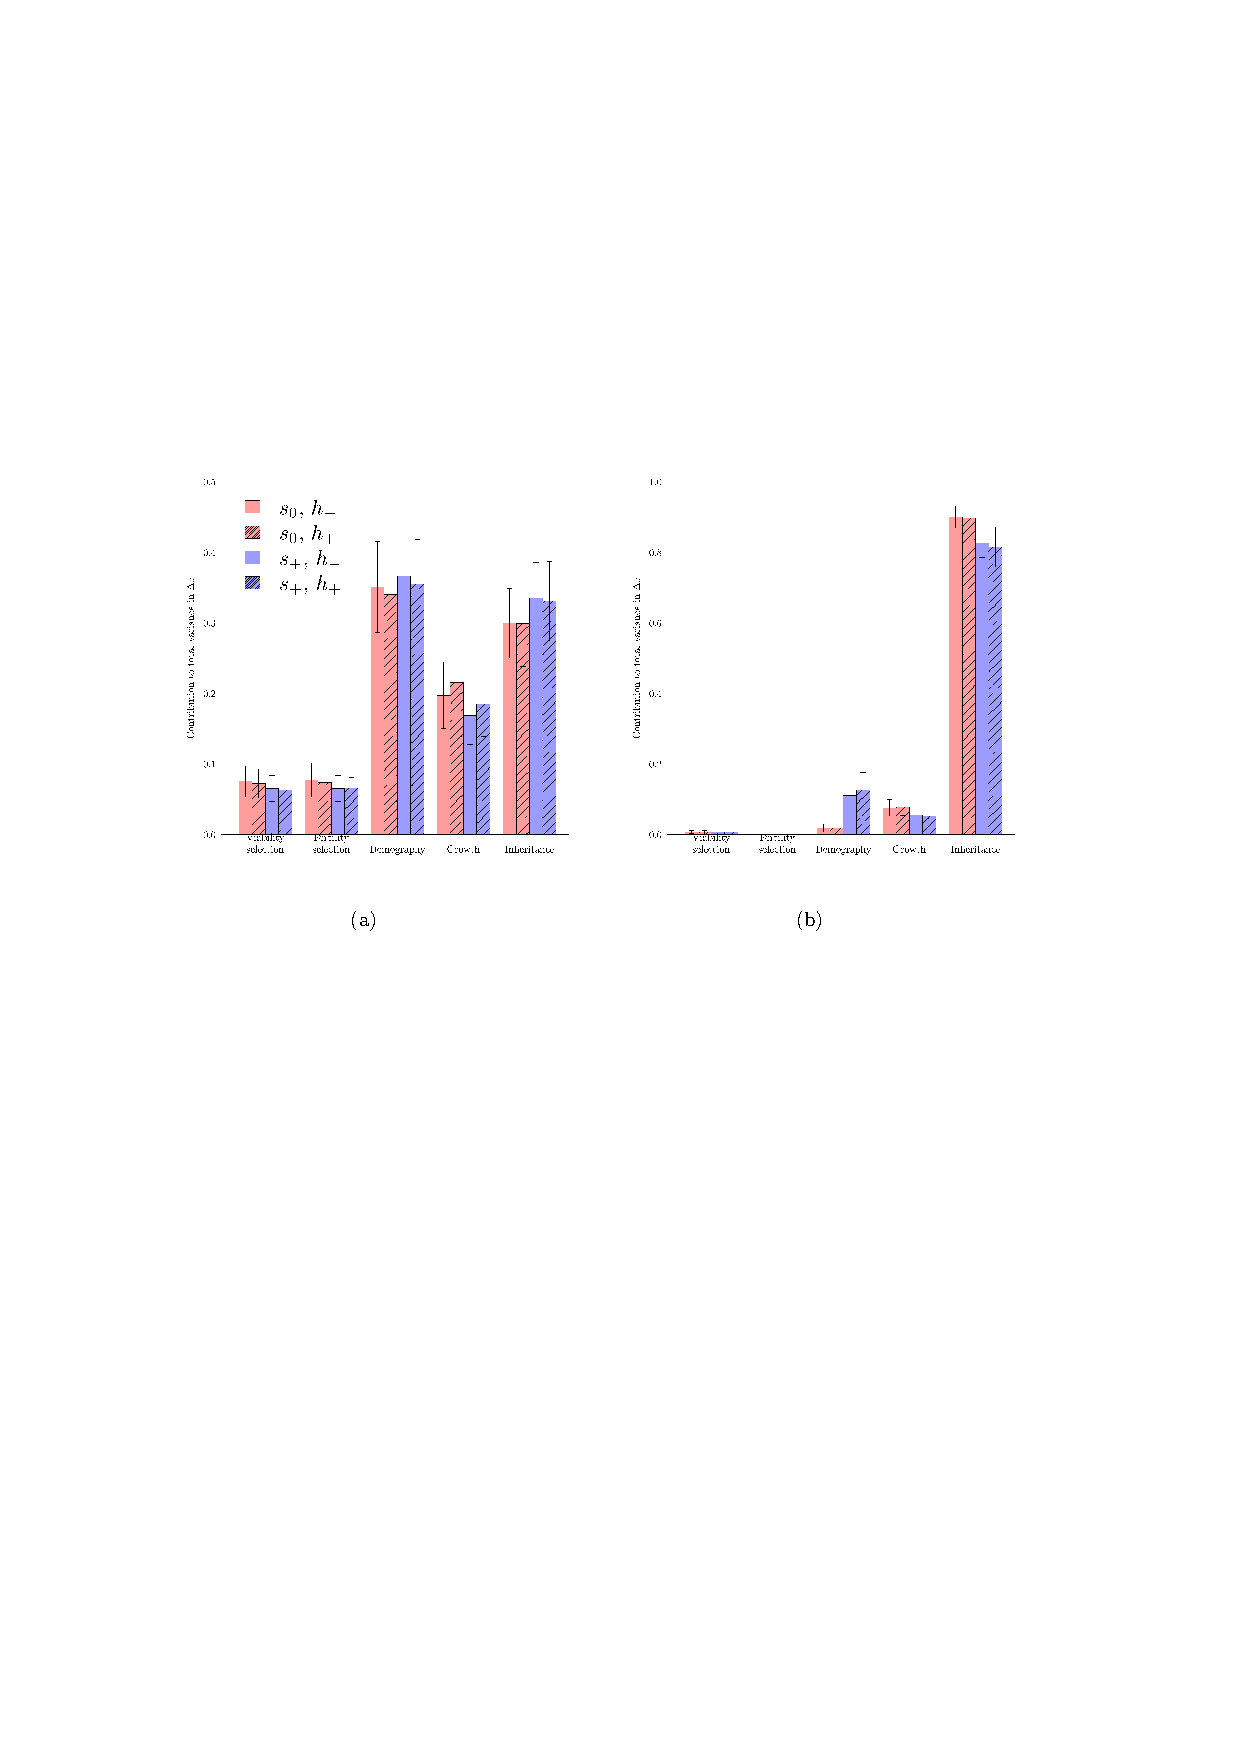
\includegraphics[width=0.9\textwidth]{Appendices/FigS5}
\caption{\footnotesize Variance partitioning of processes underlying changes in $\Delta \overline z$ according to a) the age structured Price equation, and b) integral projection models. Demography is the sum of the two demographic terms, inheritance is the sum of ODC and OMD (Appendix \ref{app:ape}). Red bars indicate scenarios without selection ($s_0$), blue bars scenarios with selection ($s_+$). Solid bars indicate scenarios with low heritability ($h_-$), shaded bars scenarios with high heritability ($h_+$). Errors bars show variation across replicates ($\pm$1 SD). Note the different scale on the y-axis in a) and b).}
\label{app:var:fig1}
\end{figure}

Although the absolute contributions to $\Delta \overline z$ are very similar (Fig. 2c and Fig. 2d), the second order contributions to $\overline z$ differ greatly between the APE and the IPM (figure \ref{app:var:fig1}). The main reason for this is that the IPM smoothens the contributions over time, through the statistical models that it is based on. A variance decomposition relies on the variation in the contributions. When the absolute values are smoothened, the outcome of the decomposition may change drastically, as observed in figure \ref{app:var:fig1}.

%From the APE application we see that changes in $\Delta \overline z$ are mainly influenced by changes in growth. This is not unexpected: the decrease in body size that we observe is mainly cause by a decreasing food availability that translates itself into a decrease in growth rates. In the IPM approach this contribution is not as prominent, instead it predicts a large contribution from survival, which seems unlikely given the stable population structure (Fig. \ref{simdata:6}). When an IPM is subjected to the APE, the interpretation of the variance decomposition cannot be done straightforwardly.

% ::

%This partitioning of variances does not take into account constant contributions to $\Delta z$. In the IPM approach the very constant (small) contribution in survival selection in figure \ref{fig:ipm-ape} has little variation, hence it explains practically none of the variation in body size (appendix X, VS). Individual growth on the contrary has large variation in the APE (figure \ref{frameworkresults:1}), leading to a large contribution in terms of explained variance (figure \ref{app:var:fig1:1}). The IPM estimates less variation in the contribution of growth, thereby leading to much less variance being explained by growth, despite very similar absolute contributions. Due to the IPM smoothing the contributions of contributions over time, it will be less precise in a variance partitioning. Furthermore, this method is blind to the direction of change. The variance partitioning (appendix X) shows for example a large contribution from fertility selection, but gives no information whether fertility selection was positive or negative. Its results should thus carefully be interpreted.